\chapter{REVIEW OF RELATED LITERATURE}

% See if this should be removed in the future
This section aims to provide the context where this study may be placed. 
Studies that have already been made in the field are to be discussed here in order to 
explain the concepts involved in enhancing genetic algorithms through the GPU and 
genetic algorithms in a game. The section will also highlight contributions not yet 
applied in the field, namely using the GPU to enhance genetic algorithms in a game.


% We need to add more material in this entire chapter
\section{Genetic Algorithms through the GPU}
\subsection{Genetic Algorithm Acceleration through GPU}
Genetic programming can be a very time-consuming process.  The members of its
populations are optimized against a fitness landscape through a fitness check. It
then tries the output or plugs it in again for a better fitness score. For a large
population, the processing power needed cannot be handled by the CPU alone. GPUs in
PCs are considered as more powerful in pure FLOPS\cite{Banzhaf09}.
For example, in the GeForce 8 Series the NVIDIA 8800 Ultra performs around 576 GFLOPS
on 128 processing elements. This equates to around 4.5 GFLOPS per element, compared
with 2.75 per core for the Blue Gene/L supercomputer.  With that kind of processing power, 
new sets of problems can be solved.  

A sample application can be found in the KDD 1999 IDS dataset, where, they had around
4 million entries.\cite{Banzhaf09}. They evaluated 10 percent of the total subset that
were given. They found out that it only took 5.86 ms to evaluate on a GPU compared to
the 43.54 ms on the CPU. They also used genetic programming to reverse engineer image
filters, i.e., find the mapping between an image and the output of a filter applied to 
it. The results were that the CPU process was 100 times slower than the GPU one.  

\subsection{Single Instruction, Multiple Threads Architechture of Nvidia Graphics Card}
A multiprocessor creates, manages, and executes threads in groups of 32 threads\cite{NVCudaPrgGuide}. 
These group of threads are called as warps. Each threads have their start at the same 
time and at the same program address. However, they have their own instruction address 
counter and register state. Thus, the threads are able to branch and execute independently.
When a multiprocessor is given one or more thread blocks to execute, it partitions into warps 
that get scheduled for execution. A warp executes one common instruction at a time. When
all 32 threads of a warp agree on their execution path, full efficiency is realized. If the threads
diverges via a data-dependent conditional branch, the warp serially executes each branch.
The threads will then converge back to the same execution path.  However, the divergence only
happens within a warp and does not affect other warps.

The single instruction, multiple threads (SIMT) architechture is similar to the single instruction,
multiple data (SIMD) vector organizations in that a single instruction controls multiple processing
elements\cite{NVCudaPrgGuide}. The difference lie in that the SIMD vectore organizations expose 
the SIMD width to the software. The SIMT instructions, on the other hand, specify the execution 
and branching behavior of a single thread. In contrast with SIMD vector machines, SIMT 
enables parallel coding for independent, scalar threads, as well as data-parallel code for 
coordinated threads. 

\begin{figure}
	\centering
		\graphicspath{{images/}}
		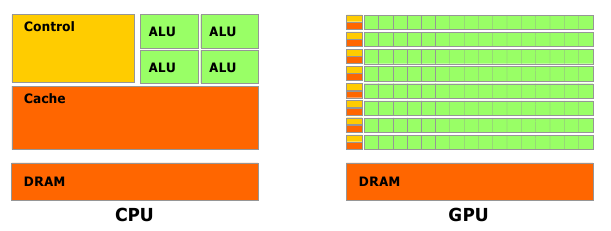
\includegraphics[width=190 pt]{cpu_gpu_blackandwhite.png}
	\caption{CPU vs GPU architechture}
	\cite{pdf:NVCudaPrgGuide}
	\label{fig:gpu_diagram}
\end{figure}


\subsection{Using CUDA in Accelerating Genetic Algorithms}
Several computers can be used to efficiently process large datasets and execute complex
and evolved programs.\cite{Harding09}. They used the spare processing power seen in the
computers in the student's laboratory. It detailed how a root computer distributed work
over a network of computers to increase processing speed and efficiency. Further
implementations were introduced in the field of genetic algorithms. NVIDIA introduced a new 
feature called the Compute Unified Device Architecture (CUDA),
a general-purpose parallel architecture with a new parallel programming model and instruction
set architecture\cite{Zhang09}. They present that with the given technology, genetic algorithms
are performed faster and more effectively. Because the GPU is much more effective in terms of primitive
operations, CUDA was introduced to take advantage of the massively parallel high-performance
computing on the GPU.  

\subsection{Implementing High Performance Genetic Programming}
However, not all genetic programs are equal in performance. Robbiliard and his colleague showed the difference between
Block genetic programming and Thread genetic programming\cite{Robbilliard09}. A Block
genetic progamming is where every genetic program is interpreted by all threads running
on a given processor. On the other hand, a Thread genetic programming is where every genetic
programs is interpreted by their own thread. They performed an experiment where
the speeds at which each setup is executed are compared. The results were that the Block genetic
programs out-performed the Thread genetic programs in every benchmark, population size and
the number of fitness cases.

\section{Genetic Algorithms Applied in Games}
\subsection{Application of Genetic Programming in a Snake Game}
Genetic algorithms in games have largely been applied in solving problems relating to
Artificial Intelligence and character behavior in games. One instance of this application
is the construction of an AI for controlling the snake in a Snake game\cite{Ehlis00}.
Tobin's approach is to alter the snake's behavior based on a gene that acts as a miniature
program that gets called at every tick of the game. Given a set of helper functions that
determined if there was danger or food in certain directions of the snake's head, the
program would construct genomes that varied in the generated tree of function calls. This
tree would then determine the snake's next actions during every tick of the game. Tobin
was able to produce genomes which created snakes that could gain scores that are close to
the maximum attainable in the game.  


A different application of genetic algorithms in a mobile version of the game of snakes
was conducted by Milan Verma and Peter McOwan in their research \cite{Verma05}. Instead
of modifying the behavior of the snake in the game, they used genetic algorithms instead
for creating whole new game levels that matched the difficulty requested by the user.
Their technique was to use genomes that determined various aspects of any single game
level and then determined the level's fitness by having the level “played” by a synthetic
game-player. The score that the synthetic game-player obtained would then determine if
the level is too easy or too hard and levels that matched the user's wants would then be
given to the user that requested it. Their study proved successful and they were able to
deliver a mobile game that could adapt to a user's needs.

\subsection{AI Game Programming}
As a proof of concept, Brian Schwab attempted to enhance the AI's ability to maneuver
the player's ship in the classic game of asteroids\cite{Schwab04}. The genomes were
constructed to represent various floating point values that would dictate different
elements for decision making. These included the distance between the ship and the asteroid,
the velocity of the ship, the velocity of the asteroid, the current angle of the rotation
of the ship and more. These values, coupled with a set of predefined functions, would then
determine how the ship would evade all the asteroids in the field. Brian was able to prove
that the ship's AI can perform better when evolved through the use of genetic algorithms as
compared to hand-modifying the AI parameters and repeatedly testing the new set of values in
the game.

\subsection{Verlet Integration}
The Verlet integration is a way of numerically describing  the movement of an object through
time\cite{Bitterli09}. There are several types of Verlet integration, Position Verlet, Velocity 
Verlet, and Leapfrog. Position Verlet gives the new position of the object by the following 
formula:

\begin{eqnarray}
Position_{new}  & = &
Position_{current} + 
(Position_{current} - Position_{old}) +
Acceleration * Timestep^2 \nonumber \\
Position_{old} & = & Position_{new} \nonumber \\
\label{Verlet}
\end{eqnarray}

The Verlet integration eliminates the need to calculate the velocity since it estimates 
the velocity using the current position and subtracting the distance with the old position. 
Through this method, the computation is fast and stable, which means a lot in enhancing the
performance of the game. Collision detection also becomes easier with the Verlet integration.
Collision is detected by finding the new position of an object and see if it intersects with
another object.


